\documentclass[12pt]{article}  % [12pt] option for the benefit of aging markers

% amssymb package contains more mathematical symbols
\usepackage{amssymb,amsthm}

% graphicx package enables you to paste in graphics
\usepackage{graphicx}
\usepackage{auto-pst-pdf}

% embed source inside latex
\usepackage[procnames]{listings}
\usepackage{color}

%%%%%%%%%%%%%%%%%%%%%%%%%%%%%%%%%
%
%    Page size commands.  Don't worry about these
%
\setlength{\textheight}{220mm}
\setlength{\topmargin}{-10mm}
\setlength{\textwidth}{150mm}
\setlength{\oddsidemargin}{0mm}

%%%%%%%%%%%%%%%%%%%%%%%%%%%%%%%%%%%%%%%%%%%%%%%%%%%%%%%%%%%%%%%
%
%    Definitions of environments for theorems etc.
%
\newtheorem{theorem}{Theorem}[section]          % Theorems numbered within sections - eg Theorem 2.1 in Section 2.
\newtheorem{corollary}[theorem]{Corollary}      % Corollaries etc. will be counted as Theorems for numbering
\newtheorem{lemma}[theorem]{Lemma}              % eg Lemma 3.1, ... Theorem 3.2, ... Corollary 3.3.
\newtheorem{proposition}[theorem]{Proposition}
\newtheorem{conjecture}[theorem]{Conjecture}

\theoremstyle{definition}
\newtheorem{definition}[theorem]{Definition}

\theoremstyle{remark}
\newtheorem{remark}[theorem]{Remark}
\newtheorem{example}[theorem]{Example} 

%%%%%%%%%%%%%%%%%%%%%%%%%%%%%%%%%%%%%%%%%%%%%%%
%
%        Preamble material specific to your essay
%
\title{Discovery Network Topology}
\author{Jiaqi Yan\\
CS542 Project\\
supervised by
Edward Chlebus}

\begin{document}
\maketitle

% \newpage                     % optional page break
\begin{abstract}
In this project, we first propose the format of topology update message for correct topology discovery.
The \textit{portion of the network seen by a router} is used to quantify the efficiency of the network update process.
A small scale network built by 6 routers is simulated to demonstrate the process of populating topology information.
The simulation, as well as the distributed discovery algorithm, should terminate when every router's \textit{topology database} is stable.
Results are shown for router $R_1$ and router $R_6$.
\end{abstract}

\newpage                     % optional page break
\tableofcontents

\newpage                     % optional page break
\section{Problem Statement}\label{s:intro}
%
% The \label command is optional, but useful.  To cross-refer to a section/theorem/equation etc.
% labelled by \label{key}, use \ref{key}.  For example: Equation (\ref{eq:key}) follows from Theorem \ref{th:key}.

In this project, we explore the problem of letting distributed routers know the entire network topology.
As the `God' of the network, we network operator have the global view of the it.
The routers, however, only knows its direct neighbors. 
Here we are considering unidirectional links.
So \textbf{neighbors} of a particular router $r$ can fall into one of two cases: the one that can be reached from $r$ and the one that can reach $r$.

The problem can be stated more formally as follows. The network topology as the adjacent matrix $AM$ is given to us.
An example is shown below:
\begin{center}
\begin{tabular}{|r|r|r|r|r|r|r|}        % 7 columns, each right-justified
\hline                                  % horizontal line between rows
 & $R_1$ & $R_2$ & $R_3$ & $R_4$ & $R_5$ & $R_6$ \\ % header row
\hline
$R_1$ &   & 3 &   &   &    & \\
\hline
$R_2$ & 4 &   & 6 &   &    & \\
\hline
$R_3$ &   &   &   & 7 &    & \\
\hline
$R_4$ &   &   &   &   & 11 & \\
\hline
$R_5$ &   &   &   &   &    & 9 \\
\hline
$R_6$ &   & 8 & 5 &   &    & \\
\hline
\end{tabular}
\end{center}
The cost from source router $s$ to destination $d$ is given as $AM[s][d]$.
Empty cell means the cost is $\infty$, meaning no link exist between router $s$ and $d$.
Every router $r$ maintain its \textbf{topology database}. 
Initially, this database contains only row $r$ and column $r$ in matrix $AM$ because
\begin{itemize}
        \item $r$ is aware the routers it can goes to, corresponding to row $AM[r][0..N-1]$
        \item $r$ knows the routers that can goes to itself, corresponding to column $AM[0..N-1][r]$
\end{itemize}
The problem is: how to let each router has the entire topology matrix?

\section{Discovery Process}

\subsection{Message Format}
The solution is simple.
Every router advertise its current known column and row in its the incomplete.
Once a router receives advertisement from other router, if the router does not have any (row, column) tuples in the messages, it inserts this information to its database.
In other words, the essential of each message is the name of the router/sender, which, playing as a \textit{key}, indicate the row index and column index this message contains.
Then goes the \textit{value}, a tuple containing the elements in the row and the elements in the column.
An advertisement from any router contains a sequence of messages if the router has more than 1 (row, column) record in its database.

\subsection{Measuring the Discovery Process}
An obvious metric is the percentage of the network topology matrix a router currently has.
For example, at the initial stage, every router only knows 1 row and 1 column of the matrix.
So everyone starts from percentage $1/N$ where $N$ is total number of routers in the network.
At iteration $n=1$, $R_2$ received messages from router $R_1$ and $R_6$; then it has 3 rows and 3 colums, which means 50\% of the network is known to $R_2$.

\section{Simulation and Termination}
We can simulate the distributed discovery process.
Simulation's basic flow is shown in Listing \ref{lst:while-loop}.

\subsection{Termination}
The discovery step is repeated until all of the routers' topology database is stable.
That is, we jump out of the while-loop when the boolean variable $updated$ is never set to $True$ when any router $r$ invokes \texttt{update\_topo()}.
The reason is simple: if every router's topology database is identical, no new information will be transferred between each other.
At this moment, all routers must have the same and correct network view, except for that something happened after the population ends.
In this case, just restart the discovery process at each router and wait for them to converge again.

\subsection{Code Structure}
Inside the while-loop, we have a scatter-gather pattern.
In the scatter phase, router $r$ will receive messages from its each neighbors $n$ who can reach $r$ directly.
In the gathering phase, each router update its topology databased by handling the received messages, stored inside its buffer.

% Python code embedding configuration
\definecolor{keywords}{RGB}{255,0,90}
\definecolor{comments}{RGB}{0,0,113}
\definecolor{red}{RGB}{160,0,0}
\definecolor{green}{RGB}{0,150,0}
\lstset{language=Python,
        basicstyle=\ttfamily\small,
        keywordstyle=\color{keywords},
        commentstyle=\color{comments},
        stringstyle=\color{red},
        showstringspaces=false,
        identifierstyle=\color{green},
        procnamekeys={def,class,True},
        frame=single,
        numbers=left,
        numbersep=5pt,
        numberstyle=\tiny\color{blue},
        rulecolor=\color{black},
        caption={Simulation Discovery Process},
        label=lst:while-loop,
        language=Python,
}
\begin{lstlisting}
while updated:
    for r in routers:
        for n in r.neighbors:
            router_n = get_router_by_name(n, routers)
            for n_name, n_row_col in router_n.topo.items():
                n_msg = (n_name, n_row_col)
                r.recv_msg(n_msg)
    updated = False
    for r in routers:
        if r.update_topo_database():
            updated = True
\end{lstlisting}

\section{Experiment Results}
In this section, the discovery progresses for router $R_1$ and $R_6$ are shown.

\subsection{Results for $R_1$}
At each iteration, the snapshot of $R_1$'s topology database is shown in Listing \ref{lst:r1}.
For example, at the 3rd iteration, $R_1$ found out 3 other routers exist in the network.
One of them is called $R6$, who can reach $R_2$ and $R_3$ with cost 8 and 5 respectively;
also this $R_6$ can be reached from another router $R_5$ with cost 9.

\lstset{basicstyle=\ttfamily\small,
        keywordstyle=\color{keywords},
        commentstyle=\color{comments},
        stringstyle=\color{red},
        showstringspaces=false,
        identifierstyle=\color{green},
        procnamekeys={def,class},
        frame=single,
        numbers=left,
        numbersep=5pt,
        numberstyle=\tiny\color{blue},
        rulecolor=\color{black},
        caption={$R_1$'s Topology at Each Iteration},
        label=lst:r1,
        language=Python}
\begin{lstlisting}
0  [  ('r1', ({'r2': 3}, {'r2': 4}))  ]
1  [  ('r1', ({'r2': 3}, {'r2': 4})), 
      ('r2', ({'r1': 4, 'r3': 6}, {'r6': 8, 'r1': 3}))  ]
2  [  ('r1', ({'r2': 3}, {'r2': 4})), 
      ('r2', ({'r1': 4, 'r3': 6}, {'r6': 8, 'r1': 3})), 
      ('r6', ({'r2': 8, 'r3': 5}, {'r5': 9}))  ]
3  [  ('r1', ({'r2': 3}, {'r2': 4})), 
      ('r2', ({'r1': 4, 'r3': 6}, {'r6': 8, 'r1': 3})), 
      ('r5', ({'r6': 9}, {'r4': 11})), 
      ('r6', ({'r2': 8, 'r3': 5}, {'r5': 9}))  ]
4  [  ('r1', ({'r2': 3}, {'r2': 4})), 
      ('r2', ({'r1': 4, 'r3': 6}, {'r6': 8, 'r1': 3})), 
      ('r4', ({'r5': 11}, {'r3': 7})), 
      ('r5', ({'r6': 9}, {'r4': 11})), 
      ('r6', ({'r2': 8, 'r3': 5}, {'r5': 9}))  ]
5  [  ('r1', ({'r2': 3}, {'r2': 4})), 
      ('r2', ({'r1': 4, 'r3': 6}, {'r6': 8, 'r1': 3})), 
      ('r3', ({'r4': 7}, {'r6': 5, 'r2': 6})), 
      ('r4', ({'r5': 11}, {'r3': 7})), 
      ('r5', ({'r6': 9}, {'r4': 11})), 
      ('r6', ({'r2': 8, 'r3': 5}, {'r5': 9}))  ]
\end{lstlisting}


\subsection{Results for $R_6$}
At each iteration, the snapshot of $R_6$'s topology database is shown in Listing \ref{lst:r6}.
For example, at the 3rd iteration, $R_1$ found out 3 other routers exist in the network.
One of them is called $R_3$, who can reach $R_4$ with cost 7;
also this $R_3$ can be reached from either router $R_6$ with cost 5 or router $R_2$ with cost 6.

\lstset{basicstyle=\ttfamily\small,
        keywordstyle=\color{keywords},
        commentstyle=\color{comments},
        stringstyle=\color{red},
        showstringspaces=false,
        identifierstyle=\color{green},
        procnamekeys={def,class},
        frame=single,
        numbers=left,
        numbersep=5pt,
        numberstyle=\tiny\color{blue},
        rulecolor=\color{black},
        caption={$R_6$'s Topology at Each Iteration},
        label=lst:r6,
        language=Python}
\begin{lstlisting}
0  [  ('r6', ({'r2': 8, 'r3': 5}, {'r5': 9}))  ]
1  [  ('r5', ({'r6': 9}, {'r4': 11})), 
      ('r6', ({'r2': 8, 'r3': 5}, {'r5': 9}))  ]
2  [  ('r4', ({'r5': 11}, {'r3': 7})), 
      ('r5', ({'r6': 9}, {'r4': 11})), 
      ('r6', ({'r2': 8, 'r3': 5}, {'r5': 9}))  ]
3  [  ('r3', ({'r4': 7}, {'r6': 5, 'r2': 6})), 
      ('r4', ({'r5': 11}, {'r3': 7})), 
      ('r5', ({'r6': 9}, {'r4': 11})), 
      ('r6', ({'r2': 8, 'r3': 5}, {'r5': 9}))  ]
4  [  ('r2', ({'r1': 4, 'r3': 6}, {'r6': 8, 'r1': 3})), 
      ('r3', ({'r4': 7}, {'r6': 5, 'r2': 6})), 
      ('r4', ({'r5': 11}, {'r3': 7})), 
      ('r5', ({'r6': 9}, {'r4': 11})), 
      ('r6', ({'r2': 8, 'r3': 5}, {'r5': 9}))  ]
5  [  ('r1', ({'r2': 3}, {'r2': 4})), 
      ('r2', ({'r1': 4, 'r3': 6}, {'r6': 8, 'r1': 3})), 
      ('r3', ({'r4': 7}, {'r6': 5, 'r2': 6})), 
      ('r4', ({'r5': 11}, {'r3': 7})), 
      ('r5', ({'r6': 9}, {'r4': 11})), 
      ('r6', ({'r2': 8, 'r3': 5}, {'r5': 9}))  ]
\end{lstlisting}

\subsection{Discovery Percentage as a function of the iteration number}
As a function of iteration, the percentage of network discovered by router $R_1$ and $R_6$ is shown in Figure \ref{fig:progress}.
The iteration number begins from 0 and ends at 6, an extra iteration to ensure that all routers in this network hold identical topology database.

\begin{figure}[h]
\centering
        \includegraphics[width=0.8\textwidth, height=0.8\textheight]{progress.ps}
\caption{Discovery Percentage as Function of Iteration for $R_1$ and $R_6$}
\label{fig:progress}
\end{figure}


%%%%%%%%%%%%%%%%%%%%%%%%%%%%%%%%%%%%%%%%%
%
%     Bibliography
%
%     Use an easy-to-remember tag for each entry - eg \bibitem{How97} for an article/book by Howie in 1997
%     To cite this publication in your text, write \cite{How97}.  To include more details such as
%     page, Chapter, Theorem numbers, use the form \cite[Theorem 6.3, page 42]{How97}.
%
%\begin{thebibliography}{99}

% 
% The usual convention for mathematical bibliographies is to list alphabetically
% by first-named author (then second, third  etc. author then date)
% websites with no author names should go by the site name
%


% Typical layout for reference to a journal article
%
%\bibitem{Bovey}
%J. D. Bovey, M. M. Dodson,                         % author(s)
%The Hausdorff dimension of systems of linear forms % article name
%{\em Acta Arithmetica}                             % journal name - italics
%{\bf 45}                                           % volume number - bold
%(1986), 337--358.                                   % (year), page range

%% Typical layout for reference to a book
%%
%\bibitem{Cassels}
%J. W. S. Cassels,                                  % author(s)
%{\em An Introduction to Diophantine Approximation},% title - italics
%Cambridge University Press, Cambridge, 1965.       % Publisher, place, date.

%% Typical layout for reference to a website
%%
%\bibitem{GAP}
%The GAP Group, GAP -- Groups, Algorithms, and Programming,  % Site name
%Version 4.5.6; 2012. % other information
%(http://www.gap-system.org)  % URL


%% Typical layout for reference to an online article
%%
%\bibitem{Howie}
%J. Howie,                                            % author(s)
%{\em Generalised triangle groups of type $(3,5,2)$}, % article name - italics
%http://arxiv.org/abs/1102.2073                       % URL
%(2011).                                              % (year)
%\end{thebibliography}

\end{document}
